\chapter{Results and Analysis} \label{7ResultsAnalysis}
This chapter provides a graphical representation of the data acquired from conducting the tests designed in the last chapter. The raw data used to generate this graphs can be accessed in Appendix \ref{ApdxData}. After the graphs their analysis is done to explain the various characteristics of the two wireless protocols according to the experimental results.

\section{\acrlong{ht} Test}
The data acquired from the different test cases of the \gls{ht} test suite is represented graphically below. The legend used for naming the test cases is same as described in section \ref{6HTdesign}.

\subsection{Graphical Representation of the Data Acquired}

Note that in figure \ref{fig:HT-dr} there are two Y-axis representing the data rate in packets per second and kilobit per second. The link layer payload of 27 bytes and 110 byte was used for BLE and 802.15.4 respectively to calculate the data rate in kbps. The data used for the plot is the median of the 10 tests conducted, each of one minute. The standard deviation of the data rate from  these 10 tests are also plotted. 
\begin{figure}[h]
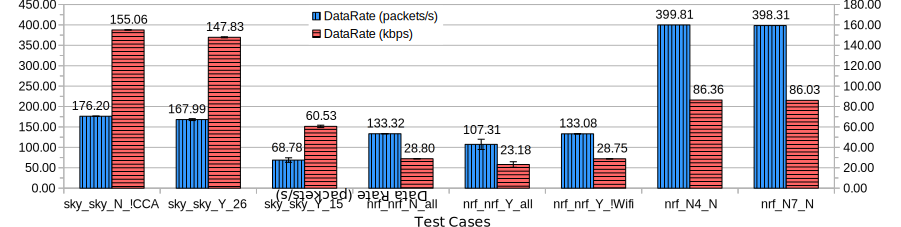
\includegraphics[width=\textwidth]{HT-dr}
\caption{Data Rate}
\label{fig:HT-dr}
\vspace{-10 pt}
\end{figure}

\begin{figure}[h]
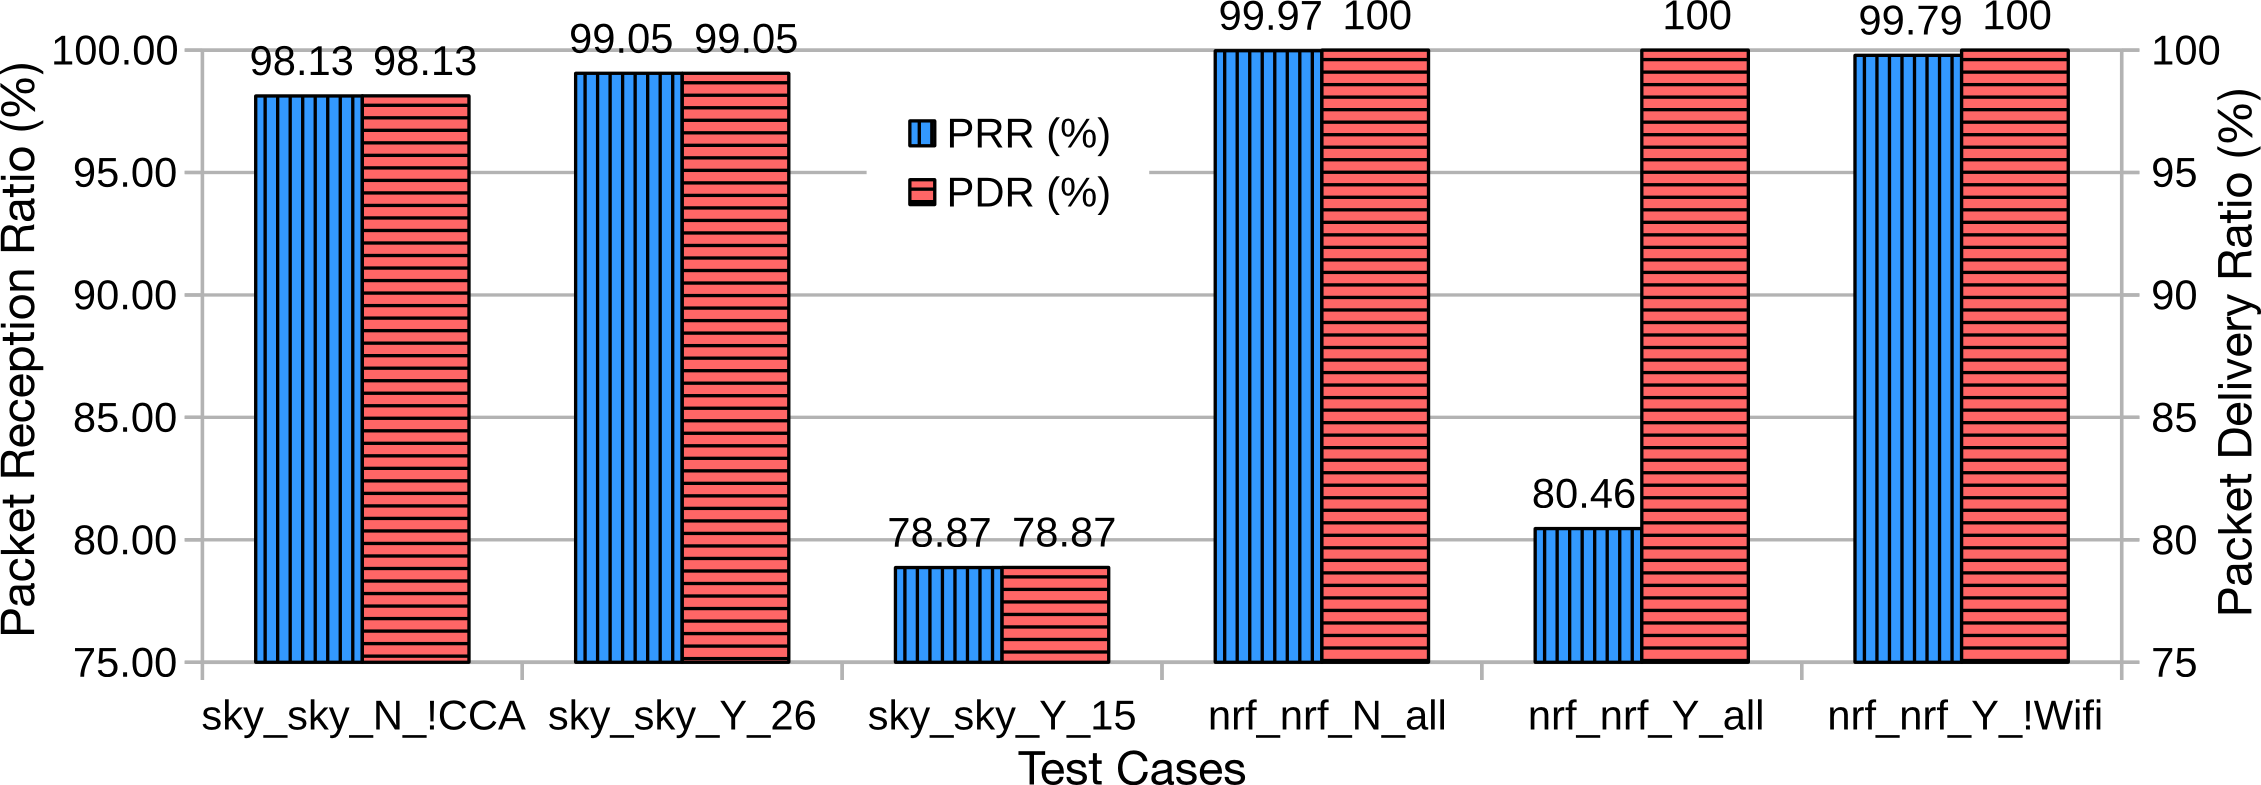
\includegraphics[width=\textwidth]{HT-r}
\caption{Reliability}
\label{fig:HT-r}
\vspace{-6 pt}
\end{figure}
The graph in figure \ref{fig:HT-r} has Y-axes from 75 to 100 \% for clearer representation of the \gls{pdr} and \gls{prr}. As mentioned in section \ref{6HTdesign} the reliability was calculate in BLE by logging the number of times the radio was switched on as this information was accessible from the SoftDevice. This allowed the calculation of \gls{prr} with one packet per connection event. Since the android devices can communicate multiple packets per connection event, the \gls{prr} could not be calculated. Hence, those test cases are not plotted.

\begin{figure}[h]
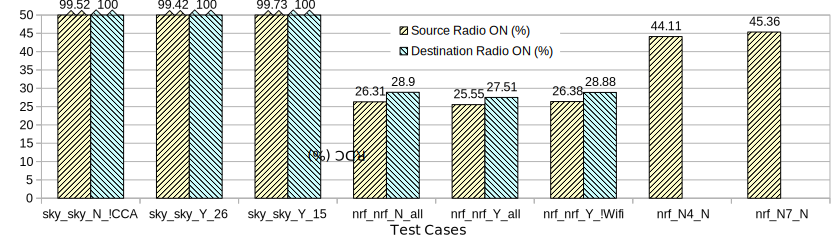
\includegraphics[width=\textwidth]{HT-ec}
\caption{Energy Consumption}
\label{fig:HT-ec}
\end{figure}

For a clearer representation of the graph, the y-axis in figure \ref{fig:HT-ec} is limited to 50\%. The break in the graph shows when Tmote-Sky uses \textasciitilde100\% of radio duty cycle. In all the tests with BLE the source node was the slave device sending the notifications, while the destination node was the master device receiving them.

There was no easy way of accessing the low level information of BLE \gls{rdc} on an Android device, so the energy consumption of these devices is not plotted. Moreover the energy consumption of such multi-purpose master device is less important than a single purpose slave device running on a meager battery.

\subsection{Analysis}
\paragraph{Data Rate}
The absolute data rate is higher in 802.15.4 than BLE although the number of packets transmitter per second is higher in BLE as seen in figure \ref{fig:HT-dr}. This is because of the higher packet size of 802.15.4 and the bit rate of transmission of BLE is four time the bit rate of 802.15.4 at 1 Mbps.

For 802.15.4 the peak data rate of 155.06 kbps is achieved when \gls{cca} is not used. The use of \gls{cca} decreased the data rate slightly. When communicating using \gls{cca} in a channel not overlapping with external interference, the data rate was 147.83 kbps. When overlapping WiFi interference was introduced, most of the transmission slots were not utilized because of backing off by \gls{cca}. Appendix \ref{ApdxData} shows that only 37\% of the transmission slots were used, dropping the data rate considerably. With this 60.53 kbps data rate was achieved, which is higher than the data rate achieved by BLE communication between nodes of PCA10000 platform in any test case. Since 802.15.4's Null-RDC tries to send a packet as soon as possible, we can approximately calculate that the inference of WiFi traffic was not present 40.1\% of the time by taking the ratio of the data rate with and without WiFi interference (60.53/147.85). \todo{can do this?}

The SoftDevice used to implement the central stack allows only one packet to be communicated per connection interval. With this the theoretical data rate that can be achieved can be found out by 

$\mbox{Data Rate  (packet/second)}=\frac{1}{\mbox{connection interval}}=\frac{1}{7.5ms}=133.33\:packet/second$

\vspace{15 pt}
$\mbox{Data Rate (kbps)}=\frac{\mbox{(bits per byte)}\times\mbox{(link layer payload in bytes)}}{\mbox{connection interval}}=\frac{8\times27}{7.5ms}=28.8\:kbps$
\vspace{10 pt}

The experimental results seen in figure \ref{fig:HT-dr} shows this is achieved accurately. When WiFi is introduced, the data rate drops from 28.8 kbps to 23.18 kbps, when all the channels are used. This is 81\% of the WiFi free data rate. Figure \ref{fig:Intf} shows that 10 out of the 37 data channels are interfered by WiFi traffic. This means that the data rate should reduce by (37-10)/37, which is about 73\% of the WiFi free data rate. The greater data rate achieved experimentally can be accounted to the fact that the WiFi traffic wasn't interfering 100\% of the time as inferred earlier with 802.15.4 data rate. 
%Considering that the 10 channels were interfered 40.1\% of the time as calculated, the data rate achievable can be calculated as $(0.401\times10/37 + 1\times27/37)\times28.8=24.2$ kbps which is closer to the achieved 23.18 kbps.

When the WiFi free channels were used the data rate recorded was close to the theoretical data rate predicted. There was negligible influence of the WiFi traffic at all for BLE communication in this case. This shows that when frequency hopping channel map is chosen to avoid the interference, there is no effect on the data rate.

Communication of the PCA10000 with a Nexus4/7 master device achieved a greater data rate of about 86 kbps or \textasciitilde400 packet/second. This is because the BLE stack in these Android devices support communication of multiple packets in a connection event, increasing the data rate achievable. With a connection interval of 7.5 ms, at an average there were around $(400\times7.5/1000)$ i.e. 3 packets of data received by the Android device per connection event.

\paragraph{Reliability}
In case of 802.15.4, the \gls{pdr} and \gls{prr} is same since it does not have any communication failure detection and retransmission mechanism. This is left to the upper layer to handle. The link layer just tries initiate communication when there is no external interference present with its \gls{cca}. Figure \ref{fig:HT-r} shows that the \gls{prr} achieved when \gls{cca} is switched off is 98.13\%, the value being high since there was little external interference. While it can be seen that without \gls{cca} the data-rate is higher, the reliability decreases. By using \gls{cca} in a WiFi free channel, the \gls{prr} is 99.05\%, which means that the \gls{cca} is effective in case of less interference in the operated channel. When there was heavy WiFi traffic in the same channel of communication, the \gls{cca} did work since only 36.82\% of the transmission slots were used. Of these transmissions the \gls{prr} was 78.87\%. This could happen when the interference starts after the carrier assessment, causing the packet to get corrupted. Here it can be seen that \gls{cca} of 802.15.4 has reduced effectiveness in case of heavy interference.

In case of \gls{ble}, figure \ref{fig:HT-r} shows that the \gls{pdr} is always 100\% since BLE employs a simple acknowledgment scheme to detect if the communication has not been successful so that the packet can be retransmitted. This ensures that the upper layers can safely assume that the link layer is completely reliable. Without WiFi interference \gls{prr} was about 99.97\%, which means that there were few retransmissions. With all the channels employed and with WiFi interference, the \gls{prr} reduced to 80.46\%. This number is not low because of the frequency hopping used by BLE, which ensures that interference in one frequency range only effects the communication happening over the channels in that frequency range. The other data channels can still keep the communication flow intact. This shows that the frequency hopping when used over the complete channel map helps in sustaining the communication when there is external interference. When only the WiFi free channels were employed, there was no influence of the WiFi interference on \gls{prr}, which was 99.79\%. This shows that when a master device has the capability of detecting external interference, it can adapt the frequency hopping channels so that there is negligible effect on the communication. Note that \gls{afh} can only help negate narrow band interference in the 2.4 GHz \gls{ism} band.

\paragraph{Energy Consumption}
As seen in figure \ref{fig:HT-ec}, the radio of Tmote-Sky nodes is used nearly 100\% the time in all the test cases of the \gls{ht} test suite. This shows that in 802.15.4 the data rate can be maximized, by choosing an appropriate \gls{rdc} layer like Null-RDC, although at the expense of energy consumption. 

When the test cases where the communication happened between PCA10000 node, the source node had \gls{rdc} between 25.5\% and 26.5\%. The destination nodes had \gls{rdc} between 27.5\% and 29\%. From this we can see that when streaming data every connection interval, the energy consumption of the master and slave is similar, with the master node being a few percent higher. The energy consumption isn't affected by the presence of external interference in this case of the stack supporting one packet per connection event. This is because the radio must switch on anyway in each connection event to detect if the communication is successful. In case multiple packets per connection interval is supported, the energy consumption for streaming of data with external interference could be lower as the connection event ends prematurely. This could not be tested with the existing setup.

In case of communication with the Android devices, the source nodes had \gls{rdc} of 44\% to 45\%. This is higher because multiple packets were communicated per connection interval, which also increased the data rate. This shows that when a master device can support communication of greater number packets per connection event, both the data rate and energy consumption increases.

\section{\acrlong{rr} Test}
The data acquired from the different test cases of the \gls{rr} test suite is represented graphically below. The legend used for naming the test cases is same as described in section \ref{6RRdesign}.
\subsection{Graphical Representation of Data Acquired}
\begin{figure}[h]
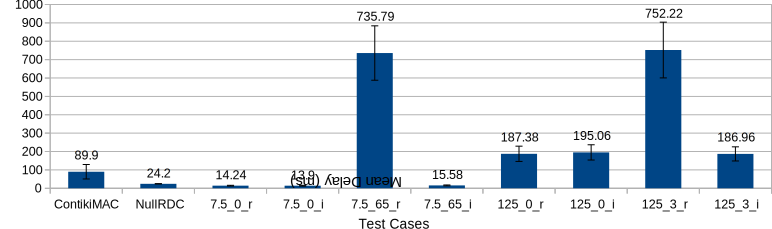
\includegraphics[width=\textwidth]{RR-l}
\caption{Latency}
\label{fig:RR-l}
\end{figure}

Figure \ref{fig:RR-l} shows the mean of the thousand measurement of latency in ms for different cases of the \gls{rr} test suite along with the standard deviation. 

\begin{figure}[h]
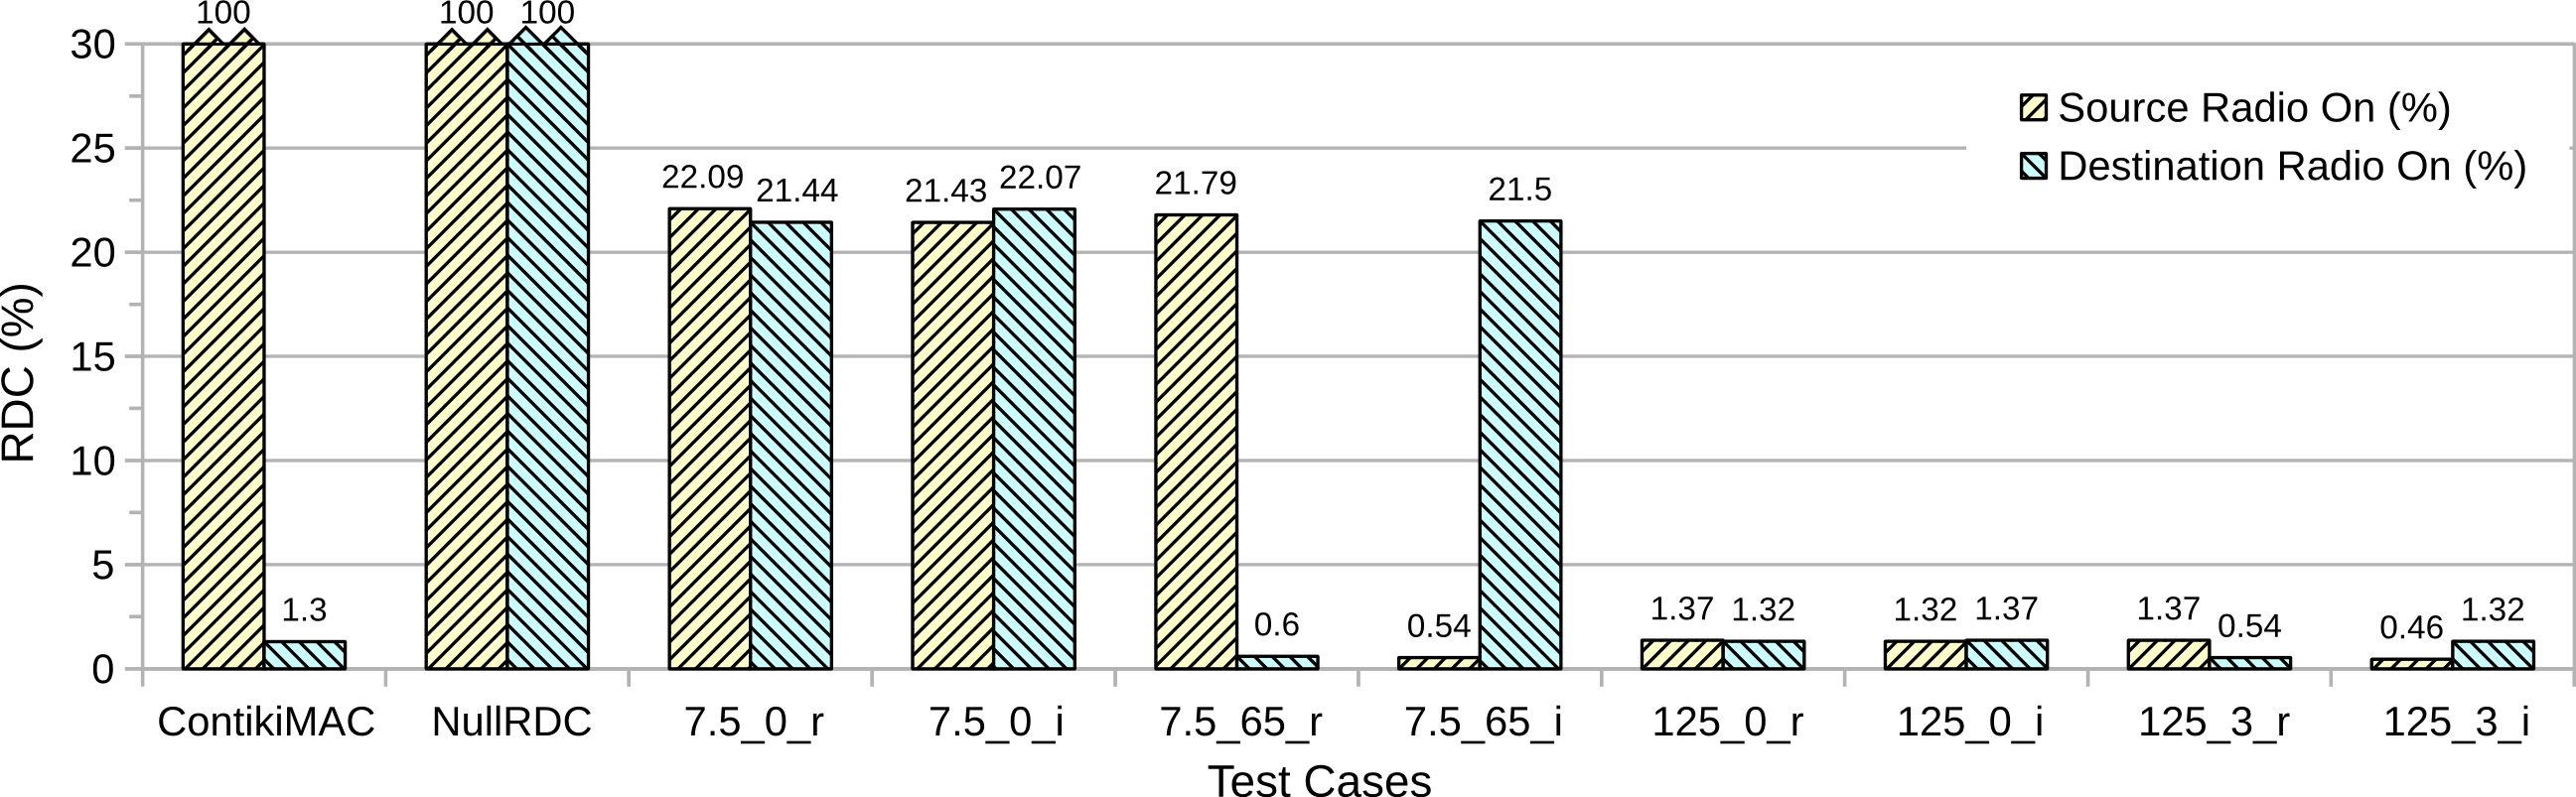
\includegraphics[width=\textwidth]{RR-ec}
\caption{Energy Consumption}
\label{fig:RR-ec}
\end{figure}

Figure \ref{fig:RR-ec} shows the energy consumption of the nodes in terms of the percentage of time the radio was switched on for the different cases of the \gls{rr} test suite. Similar to the graph for the \gls{ht} tests, this graph is limited to 30\% for clearer representation, especially of in test cases with low duty cycle.

In 802.15.4 the source and destination nodes can be identified based on who's sending and who's receiving. In case of BLE it is a bit more complicated since source and destination nodes change based on where the latency is being measured. In the tests with the master reading a packet from the slave, the master is the source while the slave is the destination. In tests with the slave sending an indication packet to the master and receiving an acknowledgment from it, the source and destination are inverted.

\begin{table}[h]
\centering
\begin{tabular}[c]{|l|l|l|l|}
\hline
Latency (ms) & Master RDC (\%) & Slave RDC (\%) & Test case \\ \hline
14.24 & 22.09 & 21.44 & 7.5\_0\_r \\ \hline
13.9 & 22.07 & 21.43 & 7.5\_0\_i \\ \hline
735.79 & 21.79 & 0.6 & 7.5\_65\_r \\ \hline
15.58 & 21.5 & 0.54 & 7.5\_65\_i \\ \hline
187.38 & 1.37 & 1.32 & 125\_0\_r \\ \hline
195.06 & 1.37 & 1.32 & 125\_0\_i \\ \hline
752.22 & 1.37 & 0.54 & 125\_3\_r \\ \hline
186.96 & 1.32 & 0.46 & 125\_3\_i \\ \hline
\end{tabular}
\caption{Latency in terms of master and slave \gls{rdc}}
\label{tbl:latVsEnergy}
\end{table}

Table \ref{tbl:latVsEnergy} shows the latency measurement from the data acquired in the \gls{rr} test in terms of BLE master and slave \gls{rdc} in different test cases. With this data the graph in figure \ref{fig:RR-l-ec} was plotted to show the various possible latency values for different master and slave's energy consumption. Note that this table and graph includes data from the BLE test cases as it is made to evaluate the impact of the various configurations on latency in terms of energy consumption.

\begin{figure}[h]
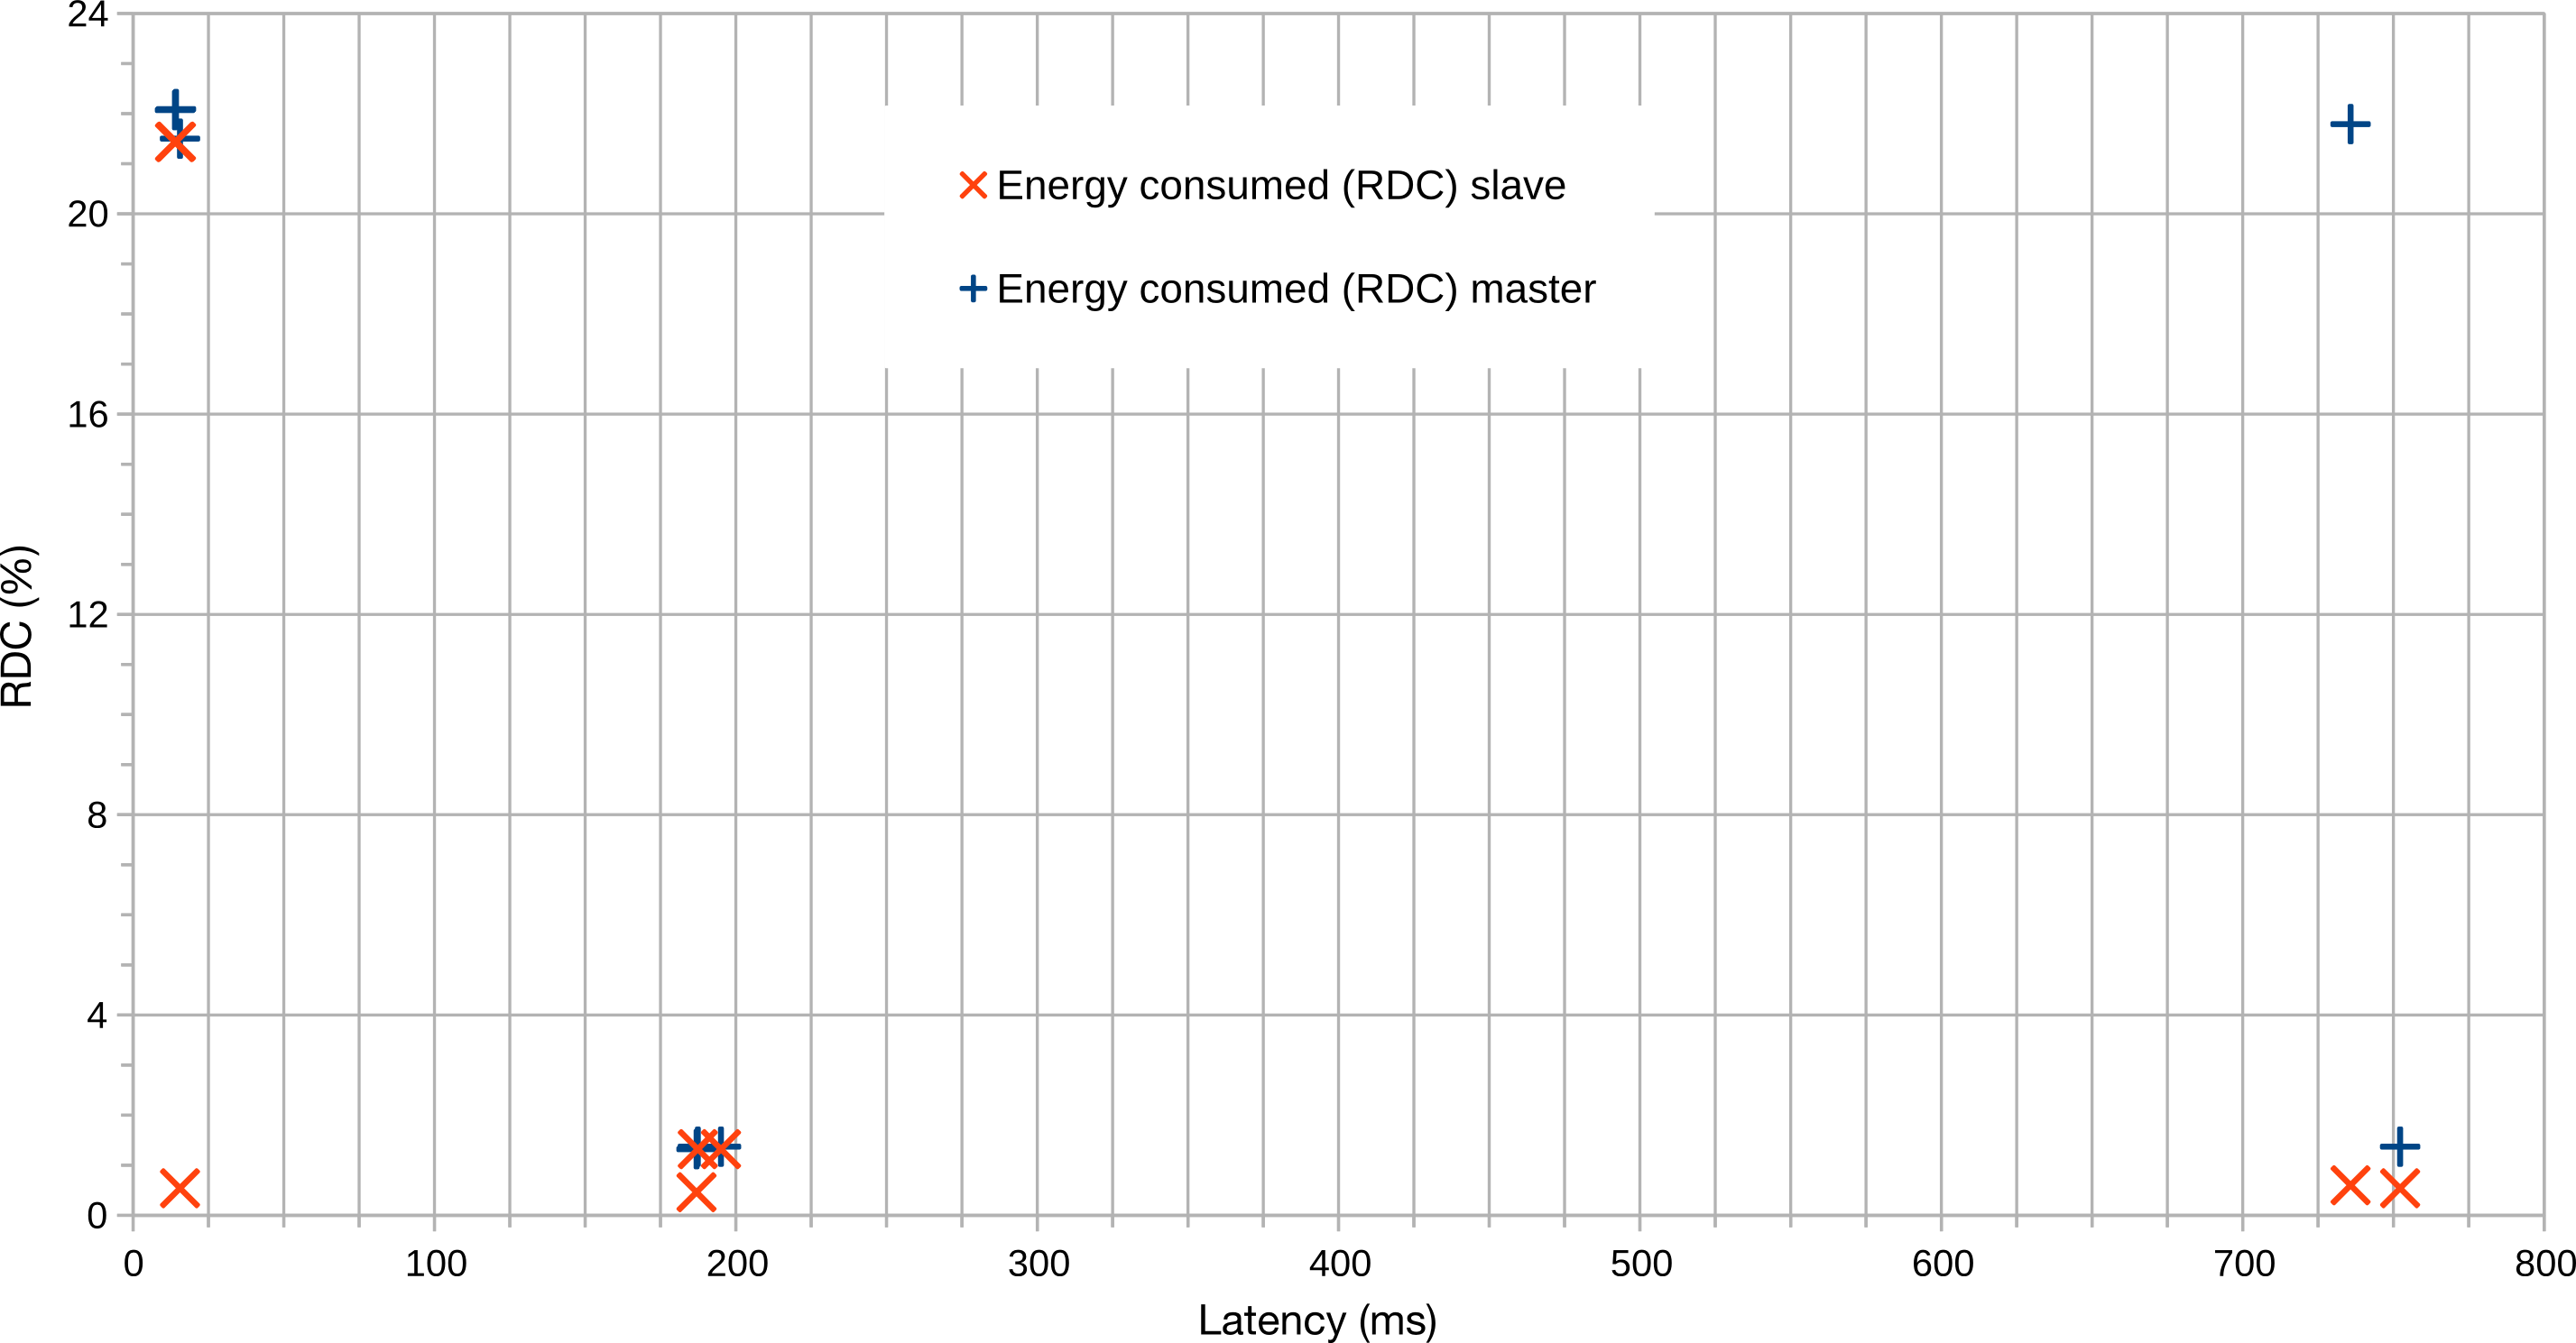
\includegraphics[width=\textwidth]{RR-l-ec}
\caption{Energy Consumption vs Latency}
\label{fig:RR-l-ec}
\end{figure}

\subsection{Analysis}
\paragraph{Latency}
The latency measurement as seen from figure \ref{fig:RR-l} can vary in the order of magnitude among different tests. The least latency can be achieved using 802.15.4 when using Null-RDC, which is about 24 ms.  When using ContikiMAC, the average latency was about 90 ms, which can be attributed to the 125 ms interval with which the receiver wakes up. In this test case where the source was assumed to be unconstrained in terms of power, it's radio was always listening, if not transmitting. This means that when the constrained destination node when ready to send the reply, the source node will be listening and get the reply immediately. This is the reason the average latency is less than the waking interval of the receiver. Note that in case both the nodes have a sleep and wake up routine, the latency would be greater than the waking interval. One disadvantage of various 802.15.4 based MAC standards is that there is no way of dynamically changing the link layer parameters. This is because there is no hierarchal master and slave concept to force particular link layer parameters.

Based on the link layer configurations used for BLE, the latency varied from a minimum of about 14 ms to a maximum of about 750 ms. The provision in BLE's link layer for changing these configurations while in a connection is an advantage since the latency can be adapted according to the requirement dynamically. The configuration of the slave latency value determines if there is any difference in the latency experienced based on whether the communication happens with a read request or an indication. With slave latency as zero, the latency of the read and indication case is almost same, with the average latency being around 14 ms with 7.5 ms connection interval and 190 ms with a connection interval of 125 ms. With a non-zero slave latency value, the read-request from the master node (client in \gls{att}) has high latency since the slave node (server at \gls{att})will not react to the master at every connection interval as it is sleeping. With a slave latency value of 65, the master node can read a value from the slave node with a latency of about 736 ms, even with a connection interval of 7.5 ms. Similarly, with a slave latency of 3 and connection interval of 125 ms, the master will read a value from the slave with a latency of about 752 ms. When using indication to communicate data to a master, the latency can be low since the slave can decide to respond to the master when necessary communicate. With a 7.5 ms connection interval and slave latency of 65, the latency is about 15 ms, which is similar to the latency experience with zero slave latency. Similarly, an indication providing the master with data experiences a latency of 187 ms with a connection interval of 125 ms and slave latency of 3. This is almost equal to the latency experienced with zero slave latency. This shows that use of indication does not effect the latency experienced to send data to a master node in a connection with non-zero slave latency.

With slave latency as zero, it can be seen that for an application layer the latency experienced is between one and two times the connection interval, the best case being close to one connection interval. This shows that a read-request communication happening in the same connection event is not possible. The read request in sent in one connection event and the requested data is sent back in the next connection event. This is because the 150 \si{\micro \second} inter frame time in a connection event is not enough for the resource constrained \glspl{mcu} respond back with the requested data.

\paragraph{Energy Consumption}
The energy consumption of the 802.15.4 source and destination node is 100\% in terms of \gls{rdc} in case of Null-RDC. This is as expected because of the nature of Null-RDC implementation. In case of ContikiMAC, the source node has 100\% \gls{rdc} while the destination has 1.3\%. The source node has this high energy consumption because it is configured so. This in accordance with the assumption of one node being unconstrained in terms of power. Usually the root node of a 802.15.4 network has access to a wall socket and gathers data from the other nodes. It is the destination node which is battery operated and has to conserve energy. 

In case of BLE, the energy consumption of the nodes which have to switch on their radio every 7.5 ms have the highest \gls{rdc} at around 21-22\%. This includes both the source and destination when the slave latency is zero and connection interval is 7.5 ms. In case the slave latency of 65 is used, the master has \gls{rdc} of around 21\%, while the slave has a \gls{rdc} of only 0.6\%. This is since the slave  can choose only to respond to the master every 66th connection interval and sleep the rest of the time, thereby creating an asymmetric architecture. Similarly when the connection interval is 125 ms and slave latency is zero, both master and slave node have 
approximately equal \gls{rdc} of 1.32 to 1.37\%. By using a slave latency of 3 and the same connection interval, the slave nodes were able to sleep for longer duration leading to the reduction of \gls{rdc} to around 0.6\%.

\paragraph{Latency vs Energy Consumption}

Figure \ref{fig:RR-l-ec} clearly showcases the flexibility available in BLE in configuring the link layer dynamically. The parameter that allows that is slave latency. A symmetric connection is created when the slave latency is zero, causing slave to respond to the master in every connection interval. This scenario will result in the latency for a read response from either the master or the slave being almost equal. Also the \gls{rdc} of the master and slave device will be similar. In this case there is a direct relation between the latency and connection interval, which means that if lower latency is required then more energy is consumed. This scenario is useful when the latency requirement for any communication started by the master is greater than that of the slave. An example for this scenario is a \gls{hid} that also provides feedback to the user, like as a game controller as a slave communicating with a gaming console as master. In this case there needs to be low latency for both the commands sent from the controller to the console, as well for the vibration feedback sent to the controller from the console. The test case that represent this in figure \ref{fig:RR-l-ec} are the ones with 7.5 ms connection interval and zero slave latency to achieve near instantaneous response.

By using a non-zero slave latency, the slave node can be sleepy by not having the responsibility to respond in every connection event. As figure \ref{fig:RR-l-ec} shows, this asymmetric connection creates a situation where the communication started from the slave has a latency as if the slave latency parameter was zero, since the master is communicating in all connection events. On the other hand, communication started by the master can experience high latency, since it has to wait till the master responds. This can be seen in the case \texttt{7.5\_65\_i} where the slave can communicate with 14 ms latency with the master while having a \gls{rdc} of only 0.54\%, although the master's radio needs to be on for about 21.5\% of the time. This scenario is useful with \gls{hid} devices such as keyboards where there is usually no feedback to be the sleepy slave devices. This will allow them to have low latency to communicate the keys pressed while allowing them to sleep when the keyboard isn't used, hence extending battery life.

\section{Evaluation with existing research}
\paragraph{Data Rate}
Considering the research that looked into the data rate achievable, the data rate achieved in this project falls well within the maximum data rate achievable\cite{Gomez2011} of 236.7 kbps. The data rate in experiments have looked at the data rate from the link layer\cite{Mikhaylov2013} or application layer\cite{Gomez2012}\cite{Mackensen2012}\cite{Kindt2014}, all of them by sending notification packets. To equalize the result with this experiment, the data rate is compared in terms of packets per second and presented in table \ref{tbl:dataRate}.

\begin{table}[h]
\centering
    \begin{tabular}[c]{|l|m{2.7cm}|l|l|}
    \hline
    Article    & Throughput (packet/second) & Devices communicating & Master device's stack \\ \hline
    This expt. & 133.3 & PCA10000 to PCA10000 & S120 v1.0.0    \\ \hline
    This expt. & 399.8 & PCA10000 to Nexus4/7 & Android 4.4.4  \\ \hline
    \cite{Gomez2012} & 365.5 & CC2540 to CC2540 (dev board) & TI BLE Stack \\ \hline
    \cite{Mackensen2012} & 250 & CC2540 to CC2540 (dev board) & TI BLE Stack \\ \hline
    \cite{Kindt2014} & 637.5 & Bluegiga BLE112 to BLE112 & Bluegiga stack \cite{MikkoSavolainen} \\ \hline
    \cite{Mikhaylov2013} & 567.6 & CC2540 to CC2540 (dev board) & TI BLE Stack v1.21 \\ \hline
    \end{tabular}
    \caption{Comparison of \gls{ble} data rate achieved}
    \label{tbl:dataRate}
\end{table}

This comparison shows that the data rate achieved is highly dependent on the BLE stack used. The BLE stack used, on both the master and slave device, determines parameters such as connection interval and packets consistently allowed to be transmitted per connection event with full application payload of 20 bytes. As seen from the table above, even though all the devices are following the BLE core specification, the limitations of the stacks for these two parameters determines the maximum data rate achievable. By improvements in the stack implementation, the data rate can be improved to reach closer to the limit of 236.7 kbps, thus extending BLE to application which require intermittent streaming of data.

This thesis project extends the research to data rate achievable in the presence of WiFi interference when using both complete and WiFi free BLE channel map. The energy consumption in terms of \gls{rdc} has been measured when sending data at maximum data rate, to two different master devices at different data rates.

\paragraph{External Interference}
As mentioned in section \ref{4ble802}, in an experiment\cite{Siekkinen2012} the \gls{prr} was measured for receiving the advertisements of a slave by a master, while varying the distance of the source of interference. Similarly, the influence of WiFi on BLE advertisement and vise versa has been evaluated for up to 21 advertisers\cite{Wyffels}. This thesis extends the research of the effect of WiFi interference on BLE in connection mode in terms of both \gls{prr} and \gls{pdr}. Although automatic \gls{afh} was not available in the test setup in this project, the effect of \gls{afh} was analyzed by manually selecting the channel map without WiFi interference. 

\paragraph{Reliability} There has been research on reliability of receiving the advertisement packets by scanners in the presence of WiFi interference\cite{Wyffels}\cite{Siekkinen2012}. To the best of the author's knowledge, this is the first experiment which finds the reliability of the link layer of BLE when in a connection. This has been looked into with and without external WiFi interference.

\paragraph{Latency}
The latency for detection of a BLE advertiser by a scanner has been extensively modeled and verified\cite{Kindt2014}\cite{Liu2012}. Latency for periodic formation of BLE connection and transfer of data has been measured\cite{Dementyev2013}, although the advertising and link layer configuration has not been detailed. The time for a connection event with sending a packet with maximum payload is measured as latency\cite{Gomez2012}. One article has measured the latency for a read-request operation, where the time measurement starts and ends with sending and receiving the data at the physical layer to/from the link-layer\cite{Mikhaylov2013}. This thesis project extends the research by exploring the influence of the link-layer parameters of connection interval and slave latency on the latency measurement for a read-request operation.

\paragraph{Energy Consumption}
Consistent with the name of the protocol, there has been extensive research on the energy consumption of a BLE devices. A recent paper has extensively and precisely modeled the energy consumption of BLE devices in during a connection and when being advertisers and scanners\cite{Kindt2014}. Various BLE \glspl{ic} have their power consumption compared in a compared\cite{Bernegger2014}. The battery life of a BLE device has been estimated for various connection and packet configuration\cite{Gomez2012}. There have been many research papers where the energy required for the different phases of a BLE transmission is accurately measured\cite{Mikhaylov2013}\cite{Siekkinen2012}\cite{Mackensen2012}\cite{liu2012energy} for the CC254x \gls{soc} from Texas Instruments.

This thesis project complements this existing research by providing an idea of the energy consumed for various scenarios, especially useful for bivariate analysis with other metrics. With the existing models available, this information in terms of \gls{rdc} can easily be converted to precise energy consumed for the platform used.

\paragraph{Comparison of BLE and 802.15.4} There has been research which compares BLE link layer with standard 802.15.4\cite{Mikhaylov2013}\cite{Siekkinen2012} and  SimpliciTI\cite{Mikhaylov2013}. To the best of our knowledge, this is the first experiment which compares BLE and 802.15.4 which uses ContikiMAC and Null-RDC \gls{mac} layer. This thesis project explores test case scenarios which are practically useful to a BLE device and application developer such as streaming data to different devices, effect of heavy WiFi interference and latency for a read-request operation, all with various link-layer configuration. 